\documentclass[11pt]{article}
\usepackage[margin=1in]{geometry}
\usepackage{amsmath,amssymb,amsthm}
\usepackage{algorithm}
\usepackage{algpseudocode}
\usepackage{booktabs}
\usepackage{hyperref}
\usepackage{tikz}
\usetikzlibrary{positioning,shapes.geometric,shapes.misc,arrows.meta}

\newtheorem{definition}{Definition}
\newtheorem{theorem}{Theorem}
\newtheorem{example}{Example}

\title{Credal Cluster Tree Elimination:\\Computing All Marginals via Two-Pass Bucket Tree Propagation}
\author{IBM Research}
\date{}

\begin{document}
\maketitle

\begin{abstract}
Credal Cluster Tree Elimination (CTE) extends bucket elimination to compute
lower and upper marginal probability bounds for \emph{all} variables in a credal
network within a single two-pass execution. The first pass (collect) is identical
to standard credal variable elimination, sending messages from leaves to root.
The second pass (distribute) propagates global information from root back to leaves.
After both passes, every bucket has sufficient information to extract its local
marginal bounds. The algorithm supports epsilon-approximate pruning at all stages,
yielding an FPTAS for all-marginals inference.
\end{abstract}

\section{Background: From Single-Query to All-Marginals}

\subsection{Bucket Elimination (Single Query)}

Standard credal variable elimination (CVE), as described in the companion document
\texttt{credal\_ve.tex}, computes bounds for a \emph{single query variable} $Z$. Given
an elimination ordering, it processes buckets from first to last. The final bucket
produces the marginal for $Z$. To query a different variable, the entire elimination
must be re-run with a different ordering.

\subsection{Bucket Tree Elimination (All Queries)}

Bucket tree elimination organizes the buckets into a \textbf{tree} and performs
\textbf{two passes}:
\begin{enumerate}
  \item \textbf{Collect (upward)}: identical to standard VE --- messages flow from
        leaves to root.
  \item \textbf{Distribute (downward)}: messages flow from root back to leaves,
        propagating global information.
\end{enumerate}
After both passes, every bucket has access to the full joint information, enabling
extraction of all marginals simultaneously.

This is equivalent to the junction tree (cluster tree) algorithm of
Lauritzen and Spiegelhalter (1988), viewed through the bucket elimination framework
of Dechter (1999).

\section{Potentials (Recap)}

A \textbf{potential} $\phi(\mathbf{Y})$ is a finite set of non-negative real-valued
functions over the joint domain of variables $\mathbf{Y}$. The three operations are:
\begin{itemize}
  \item \textbf{Combine}: $\phi \cdot \psi = \{f \cdot g : f \in \phi, g \in \psi\}$
  \item \textbf{Marginalize}: $\sum_X \phi = \{\sum_x f : f \in \phi\}$
  \item \textbf{Prune}: remove dominated functions (exact or $\varepsilon$-approximate)
\end{itemize}

\section{Algorithm}

\subsection{Step 1: Bucket Tree Construction}

Given an elimination ordering $\mathbf{o} = (X_1, X_2, \dots, X_n)$ and a set of
initial potentials (one per credal factor plus evidence indicators):

\begin{enumerate}
  \item \textbf{Assign potentials to buckets.} Each potential is assigned to the
        bucket of the first variable in $\mathbf{o}$ that appears in the potential's
        scope.
  \item \textbf{Determine parent--child relationships.} For each bucket $X_i$,
        compute the \emph{message scope}: the union of scopes of all potentials in
        the bucket (including received messages), minus $X_i$ itself. The
        \textbf{parent} of $X_i$ is the next variable in $\mathbf{o}$ that appears
        in this message scope. The message scope is propagated to the parent's
        effective scope.
\end{enumerate}

The result is a rooted tree where the last variable in the ordering is the root.

\subsection{Step 2: Collect Pass (Upward)}

Process buckets in elimination order (leaves to root). At each bucket $X_i$:
\begin{enumerate}
  \item \textbf{Gather}: local potentials $+$ upward messages $\lambda_{X_j}$ from
        all children $X_j$.
  \item \textbf{Combine}: $\psi_i = \prod \{\text{gathered potentials}\}$.
  \item \textbf{Marginalize}: $\lambda_{X_i} = \sum_{X_i} \psi_i$.
  \item \textbf{Prune}: $\lambda_{X_i} \gets \mathrm{prune}(\lambda_{X_i})$.
  \item \textbf{Send} $\lambda_{X_i}$ to the parent bucket.
\end{enumerate}

This is identical to standard CVE. After the collect pass, the root bucket
has ``seen'' all information.

\subsection{Step 3: Distribute Pass (Downward)}

Process buckets in \emph{reverse} elimination order (root to leaves). At each
bucket $X_i$, for each child $X_j$:
\begin{enumerate}
  \item \textbf{Gather}: the downward message $\pi_{X_i}$ from $X_i$'s own parent
        $+$ local potentials in $X_i$'s bucket $+$ upward messages from all children
        of $X_i$ \emph{except} $X_j$.
  \item \textbf{Combine}: $\psi = \prod \{\text{gathered potentials}\}$.
  \item \textbf{Marginalize}: $\pi_{X_j} = \sum_{X_i} \psi$ (sum out $X_i$).
  \item \textbf{Prune}: $\pi_{X_j} \gets \mathrm{prune}(\pi_{X_j})$.
  \item \textbf{Send} $\pi_{X_j}$ to child $X_j$.
\end{enumerate}

After the distribute pass, every bucket has received information from the rest
of the network via its parent's downward message.

\subsection{Step 4: Extract All Marginals}

At each bucket $X_i$, the full information is:
\[
  \Phi_i = \underbrace{\text{local potentials}}_{\text{assigned in Step~1}}
  \;\cdot\; \underbrace{\prod_{j \in \mathrm{children}(i)} \lambda_{X_j}}_{\text{from collect}}
  \;\cdot\; \underbrace{\pi_{X_i}}_{\text{from distribute}}.
\]
Marginalize out all variables except $X_i$, then normalize each function and
take componentwise min/max for the lower/upper bounds.

\subsection{Pseudocode}

\begin{algorithm}[H]
\caption{Credal Cluster Tree Elimination (CTE)}
\label{alg:cte}
\begin{algorithmic}[1]
\Require Extreme points, evidence $\mathbf{Y} = \mathbf{y}$, elimination heuristic,
         optional $\varepsilon$
\Ensure Bounds $[\underline{P}(X_i{=}x),\; \overline{P}(X_i{=}x)]$ for \textbf{all}
        variables $X_i$ and states $x$
\Statex
\State Build potentials from extreme points and evidence indicators
\State Compute elimination ordering $\mathbf{o}$
\State Build bucket tree: assign potentials, determine parent--child
\Statex
\Comment{\textsc{Collect (Upward)}}
\For{each $X_i$ in $\mathbf{o}$ (leaves to root)}
  \State $\psi_i \gets \prod\{\text{local pots} \cup \{\lambda_{X_j} : j \in \mathrm{ch}(i)\}\}$
  \State $\lambda_{X_i} \gets \mathrm{prune}\bigl(\sum_{X_i} \psi_i\bigr)$
  \State Send $\lambda_{X_i}$ to parent
\EndFor
\Statex
\Comment{\textsc{Distribute (Downward)}}
\For{each $X_i$ in reverse $\mathbf{o}$ (root to leaves)}
  \For{each child $X_j$ of $X_i$}
    \State $\psi \gets \prod\{\pi_{X_i},\;\text{local pots},\;
           \{\lambda_{X_k} : k \in \mathrm{ch}(i) \setminus \{j\}\}\}$
    \State $\pi_{X_j} \gets \mathrm{prune}\bigl(\sum_{X_i} \psi\bigr)$
    \State Send $\pi_{X_j}$ to child $X_j$
  \EndFor
\EndFor
\Statex
\Comment{\textsc{Extract Marginals}}
\For{each variable $X_i$}
  \State $\Phi_i \gets \prod\{\text{local pots},\;
         \{\lambda_{X_j} : j \in \mathrm{ch}(i)\},\; \pi_{X_i}\}$
  \State $\phi_i \gets \sum_{\mathbf{Y} \setminus \{X_i\}} \Phi_i$
  \State $\underline{P}(X_i{=}x) \gets \min_{f \in \phi_i} f(x)/\sum_{x'} f(x')$
  \State $\overline{P}(X_i{=}x) \gets \max_{f \in \phi_i} f(x)/\sum_{x'} f(x')$
\EndFor
\end{algorithmic}
\end{algorithm}

%% ================================================================
\section{Detailed Example: Alarm Network}
%% ================================================================

We trace CTE on the alarm network (\texttt{alarm.lcn}) with variables $E$, $B$, $A$,
$CD$ and elimination ordering $\mathbf{o} = (E, B, A, CD)$.

\subsection{Bucket Tree}

\begin{center}
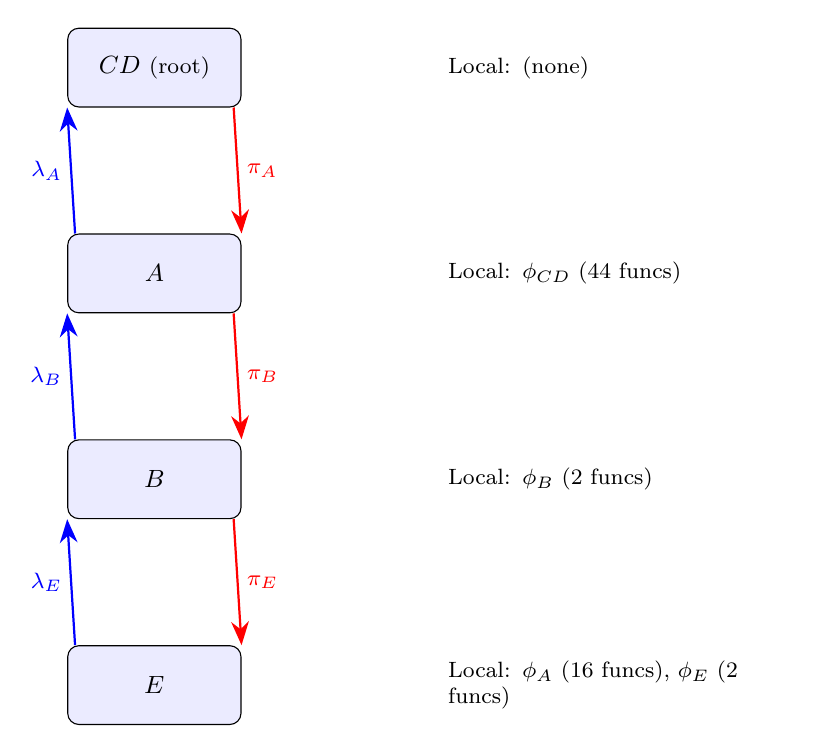
\begin{tikzpicture}[
  bucket/.style={rectangle, draw, rounded corners, minimum width=22mm,
                 minimum height=10mm, font=\small, fill=blue!8},
  msg/.style={-{Stealth[length=3mm]}, thick},
  lbl/.style={font=\footnotesize, fill=white, inner sep=1pt},
  node distance=16mm
]
  % Buckets (bottom to top = elimination order)
  \node[bucket] (E) {$E$};
  \node[bucket, above=of E] (B) {$B$};
  \node[bucket, above=of B] (A) {$A$};
  \node[bucket, above=of A] (CD) {$CD$ \footnotesize(root)};

  % Upward messages (left side)
  \draw[msg, blue] (E.north west) ++(0.1,0) -- node[lbl, left=2pt] {$\lambda_E$} (B.south west);
  \draw[msg, blue] (B.north west) ++(0.1,0) -- node[lbl, left=2pt] {$\lambda_B$} (A.south west);
  \draw[msg, blue] (A.north west) ++(0.1,0) -- node[lbl, left=2pt] {$\lambda_A$} (CD.south west);

  % Downward messages (right side)
  \draw[msg, red] (CD.south east) ++(-0.1,0) -- node[lbl, right=2pt] {$\pi_A$} (A.north east);
  \draw[msg, red] (A.south east) ++(-0.1,0) -- node[lbl, right=2pt] {$\pi_B$} (B.north east);
  \draw[msg, red] (B.south east) ++(-0.1,0) -- node[lbl, right=2pt] {$\pi_E$} (E.north east);

  % Local potentials (annotations)
  \node[right=25mm of E, font=\footnotesize, text width=42mm, align=left]
    {Local: $\phi_A$ (16 funcs), $\phi_E$ (2 funcs)};
  \node[right=25mm of B, font=\footnotesize, text width=42mm, align=left]
    {Local: $\phi_B$ (2 funcs)};
  \node[right=25mm of A, font=\footnotesize, text width=42mm, align=left]
    {Local: $\phi_{CD}$ (44 funcs)};
  \node[right=25mm of CD, font=\footnotesize, text width=42mm, align=left]
    {Local: (none)};
\end{tikzpicture}
\end{center}

\noindent The bucket tree structure:
\begin{center}
\begin{tabular}{lccll}
\toprule
\textbf{Bucket} & \textbf{Parent} & \textbf{Children} & \textbf{Local Potentials} & \textbf{Funcs} \\
\midrule
$E$ & $B$ & --- & $\phi_A$: scope $\{A,B,E\}$; $\phi_E$: scope $\{E\}$ & 16, 2 \\
$B$ & $A$ & $\{E\}$ & $\phi_B$: scope $\{B\}$ & 2 \\
$A$ & $CD$ & $\{B\}$ & $\phi_{CD}$: scope $\{CD,A\}$ & 44 \\
$CD$ & --- (root) & $\{A\}$ & (none) & 0 \\
\bottomrule
\end{tabular}
\end{center}

The factor $\phi_A$ (scope $\{A,B,E\}$) is assigned to bucket $E$ because $E$ is the
first variable in the ordering that appears in $\phi_A$'s scope. Similarly, $\phi_{CD}$
(scope $\{CD,A\}$) goes to bucket $A$.

\subsection{Collect Pass (Upward Messages)}

\paragraph{Bucket $E$:}
Combine $\phi_A$ ($16$ funcs) $\times$ $\phi_E$ ($2$ funcs) = $32$ functions over
$\{A, B, E\}$. Marginalize out $E$:
\[
  \lambda_E(\cdot) = \sum_e \psi_E(A, B, e), \qquad \text{scope: } \{A, B\}, \quad 32 \text{ functions.}
\]
After pruning: 32 functions remain. Each function $f_k(A, B)$ is a $2 \times 2$ array,
e.g.:
\[
  f_0 = \begin{pmatrix} 0.860 & 0.000 \\ 0.140 & 1.000 \end{pmatrix}, \quad
  f_1 = \begin{pmatrix} 0.908 & 0.000 \\ 0.092 & 1.000 \end{pmatrix}, \quad \dots
\]
(rows = $A \in \{0,1\}$, columns = $B \in \{0,1\}$).

$\lambda_E$ is sent to parent bucket $B$.

\paragraph{Bucket $B$:}
Combine $\phi_B$ ($2$ funcs) $\times$ $\lambda_E$ ($32$ funcs) = $64$ functions over
$\{A, B\}$. Marginalize out $B$:
\[
  \lambda_B(A) = \sum_b \psi_B(A, b), \qquad \text{scope: } \{A\}, \quad
  59 \text{ functions (after pruning).}
\]
Example functions: $f_0 = [0.688, 0.312]$, $f_1 = [0.726, 0.274]$, \dots

$\lambda_B$ is sent to parent bucket $A$.

\paragraph{Bucket $A$:}
Combine $\phi_{CD}$ ($44$ funcs) $\times$ $\lambda_B$ ($59$ funcs) = $2596$ functions
over $\{CD, A\}$. Marginalize out $A$:
\[
  \lambda_A(CD) = \sum_a \psi_A(CD, a), \qquad \text{scope: } \{CD\}, \quad
  2584 \text{ functions (after pruning).}
\]

$\lambda_A$ is sent to root bucket $CD$.

\paragraph{Bucket $CD$ (root):}
No local potentials. Combines $\lambda_A$ and marginalizes $CD$: $\lambda_{CD}$
is a scalar (scope $\emptyset$), 352 functions. This is the normalization constant.

\subsection{Distribute Pass (Downward Messages)}

\paragraph{Root $CD \to A$:}
The root has no parent message and no local potentials. The downward message to $A$
is trivial:
\[
  \pi_A = \text{scalar potential with 1 function: } f_0 = [4.0].
\]
This scalar acts as a normalization factor.

\paragraph{$A \to B$:}
Combine $\pi_A$ (1 func) $\times$ $\phi_{CD}$ (44 funcs, local to $A$) =
44 functions over $\{CD, A\}$. Marginalize out $A$:
\[
  \pi_B(CD) = \sum_a \psi(CD, a), \qquad \text{scope: } \{CD\}, \quad 44 \text{ functions.}
\]
$\pi_B$ carries information from the $CD$ factor ``above'' $B$ in the tree.

\paragraph{$B \to E$:}
Combine $\pi_B$ (44 funcs) $\times$ $\phi_B$ (2 funcs, local to $B$) =
88 functions. Marginalize out $B$:
\[
  \pi_E(CD) = \sum_b \psi(CD, b), \qquad \text{scope: } \{CD\}, \quad 60 \text{ functions.}
\]
$\pi_E$ tells bucket $E$ what the rest of the network (above $E$) ``thinks'' about $CD$.

\subsection{Marginal Extraction}

At each bucket, combine all available information:

\paragraph{Bucket $E$:}
$\Phi_E = \phi_A \cdot \phi_E \cdot \pi_E$. Marginalize out $A, B, CD$ to get
$\phi(E)$. Normalize each function, take min/max:
\[
  P(E{=}0) \in [0.9000, 0.9500], \quad P(E{=}1) \in [0.0500, 0.1000].
\]

\paragraph{Bucket $B$:}
$\Phi_B = \phi_B \cdot \lambda_E \cdot \pi_B$. Marginalize out $A, CD$:
\[
  P(B{=}0) \in [0.8000, 0.9000], \quad P(B{=}1) \in [0.1000, 0.2000].
\]

\paragraph{Bucket $A$:}
$\Phi_A = \phi_{CD} \cdot \lambda_B \cdot \pi_A$. Marginalize out $CD$:
\[
  P(A{=}0) \in [0.6880, 1.0000], \quad P(A{=}1) \in [0.0000, 0.3120].
\]

\paragraph{Bucket $CD$ (root):}
$\Phi_{CD} = \lambda_A$ (only child message, no parent). Already over $\{CD\}$:
\[
  P(CD{=}k) \in [0.0, 1.0] \text{ for all } k \in \{0,1,2,3\}.
\]
The wide bounds for $CD$ reflect the large number of extreme points (11 for $A{=}1$)
and the vacuous prior.

\subsection{Summary of Messages}

\begin{center}
\begin{tabular}{llcl}
\toprule
\textbf{Message} & \textbf{Direction} & \textbf{Scope} & \textbf{\# Functions} \\
\midrule
$\lambda_E$ & $E \to B$ (up) & $\{A, B\}$ & 32 \\
$\lambda_B$ & $B \to A$ (up) & $\{A\}$ & 59 \\
$\lambda_A$ & $A \to CD$ (up) & $\{CD\}$ & 2584 \\
$\lambda_{CD}$ & root (up) & $\emptyset$ & 352 \\
\midrule
$\pi_A$ & $CD \to A$ (down) & $\emptyset$ & 1 \\
$\pi_B$ & $A \to B$ (down) & $\{CD\}$ & 44 \\
$\pi_E$ & $B \to E$ (down) & $\{CD\}$ & 60 \\
\bottomrule
\end{tabular}
\end{center}

\section{Epsilon Approximation}

The $\varepsilon$-approximate version replaces exact pruning with $\varepsilon$-pruning
at \textbf{all three stages}:
\begin{enumerate}
  \item After each upward message is marginalized (collect pass).
  \item After each downward message is marginalized (distribute pass).
  \item After combining all information at each bucket (marginal extraction).
\end{enumerate}

\begin{definition}[$\varepsilon$-Pruning in CTE]
A function $f$ is removed from a potential if there exists another function $g$ such
that $g(\mathbf{y}) \geq f(\mathbf{y}) - \varepsilon$ for all $\mathbf{y}$.
\end{definition}

Since $\varepsilon$-pruning is applied in both passes, the effective error at any bucket
is bounded by $O(\varepsilon \times d)$ where $d$ is the bucket's depth in the tree.
For the alarm network:

\begin{center}
\begin{tabular}{lcccc}
\toprule
& $P(E{=}1)$ & $P(B{=}1)$ & $P(A{=}1)$ & Time (s) \\
\midrule
Exact ($\varepsilon{=}0$) & $[0.05, 0.10]$ & $[0.10, 0.20]$ & $[0.00, 0.31]$ & 50.0 \\
$\varepsilon{=}0.01$ & $[0.05, 0.10]$ & $[0.10, 0.20]$ & $[0.00, 0.31]$ & 11.7 \\
\bottomrule
\end{tabular}
\end{center}

The $\varepsilon$-approximate version is $4\times$ faster with identical bounds on this
small network. On larger networks, the speedup from controlling potential cardinality
growth is more dramatic.

\begin{theorem}[FPTAS for All Marginals]
For credal networks of bounded treewidth $w^*$ and bounded variable cardinality $k$,
the $\varepsilon$-approximate CTE runs in time polynomial in the number of variables
$n$, $1/\varepsilon$, and $k^{w^*}$, and produces bounds within $O(n\varepsilon)$ of
the exact bounds for all variables simultaneously.
\end{theorem}

\section{Comparison with Single-Query VE}

\begin{center}
\begin{tabular}{lcc}
\toprule
\textbf{Property} & \textbf{CVE (single query)} & \textbf{CTE (all marginals)} \\
\midrule
Passes & 1 (upward only) & 2 (upward + downward) \\
Queries per run & 1 & All $n$ variables \\
Total work for $n$ queries & $O(n)$ runs & 1 run \\
Message storage & Not needed & Store all $\lambda$, $\pi$ \\
Space & $O(C \cdot k^{w^*})$ & $O(n \cdot C \cdot k^{w^*})$ \\
\bottomrule
\end{tabular}
\end{center}

CTE is preferred when bounds on multiple or all variables are needed. CVE is
preferred for a single query, as it avoids the overhead of the distribute pass
and message storage.

\section{References}

\begin{enumerate}
\item R.\ Dechter. Bucket elimination: A unifying framework for reasoning.
      \emph{Artificial Intelligence}, 113:41--85, 1999.
\item K.\ Kask, R.\ Dechter, J.\ Larrosa, F.G.\ Cozman. Bucket-tree elimination
      for automated reasoning. Technical report, UCI, 2001.
\item S.L.\ Lauritzen, D.J.\ Spiegelhalter. Local computations with probabilities
      on graphical structures. \emph{JRSS-B}, 50(2):157--224, 1988.
\item D.D.\ Mau\'a, F.G.\ Cozman. Thirty years of credal networks.
      \emph{IJAR}, 126:133--157, 2020.
\item D.D.\ Mau\'a, C.P.\ de Campos, M.\ Zaffalon. Solving limited memory
      influence diagrams. \emph{JAIR}, 44:97--140, 2012.
\end{enumerate}

\end{document}
